\documentclass{article}
\usepackage{listings}
\usepackage{graphicx}

\newcommand{\SolutionName}{Invariants}
\newcommand{\ProjectName}{Invariants}

\newcommand{\code}[1]{\lstinline{#1}}

\title{\ProjectName{} Runtime Checking Example}
\date{}


\begin{document}
\maketitle

\begin{abstract}
This example shows the runtime checking of invariants.
It also points out a subtle issue of when an invariant check
is {\em not} done.
The example consists of three classes: a base class
\code{BasicBankAccount}, a subtype \code{WallStreetAccount}, and
a client, \code {Client} that creates bank accounts and calls methods on them.
\end{abstract}

\newcommand\codefamily\sffamily
\lstset{language={[Sharp]C},mathescape=true,flexiblecolumns=true,morekeywords={Requires,Ensures,Invariant},basicstyle=\codefamily\small,literate={->}{{$\rightarrow$}}{2}{<<}{{$\langle$}}{2}{>>}{{$\rangle$}}{2}{!}{{\textbf{!}}}{2},frame=lines,moredelim=[is][\itshape]{@}{@},captionpos=b,numberstyle=\tiny,stepnumber=1,numbersep=2pt}

\section{Adding the Contract Library Reference}
If you are using Visual Studio 2008, or if you for 
some reason want to target a pre-v4 .NET runtime, then you need to:
\begin{itemize}
\item Change the target framework of the project.
\item Manually add a reference to Microsoft.Contracts.dll
\end{itemize}
Otherwise, you may skip this section and go directly the next section!

To add the reference, open the
\textsf{\SolutionName{}} solution and right-click on
\textsf{References} in the \textsf{\ProjectName{}} project and
select \textsf{Add Reference}. Find the \textsf{Microsoft.Contracts}
library in the \textsf{.NET} tab as shown below and click OK.
\begin{center}
  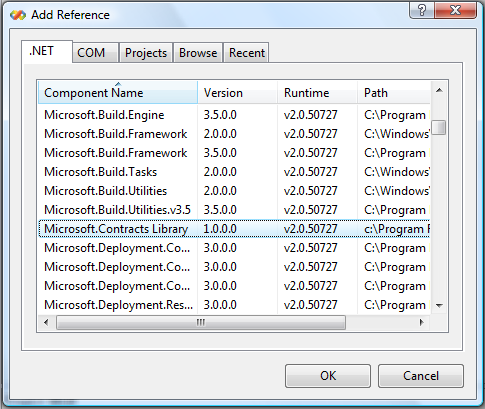
\includegraphics[width=.7\columnwidth]{../Common/addRef.png}
\end{center}



\section{Sample Walkthrough}
\label{sec:start}

Go to the Properties of project
\textsf{BasicBankAccount}, select the Code Contracts pane (at the bottom), and enable runtime
checking by clicking on the runtime checking box, as shown in this screenshot:
\begin{center}
  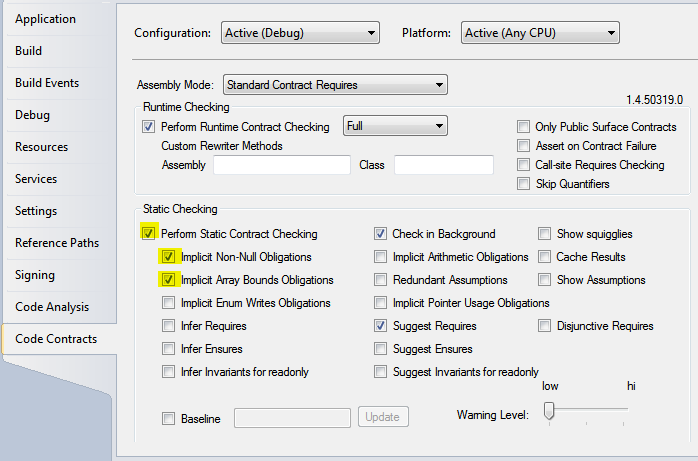
\includegraphics[width=.8\columnwidth]{ex1.png}
\end{center}

Then build the entire solution. The build should succeed.
Now let's look at some of the code in the solution.

First, take a look at \code{MainStreet.cs} which contains the very simple
class \code{BankAccount}.
It has one method for putting money into the account, \code{Deposit}, another
for removing money from the account, \code{Withdraw}, and a property, \code{Balance}, that has
only a getter for returning the amount of money that is in the account.

What is different (aside from the contracts in each of those methods) is that an object invariant
has been added to the class, a method named \code{GoodAccount}.
(The full details about invariant methods and how to write them can be found in the general documentation.)
This method gets checked at the end of every public method in the class.

Now run the program by, e.g., pressing \textsf{F5} to start the debugger.
You should see the following ``assert" dialog box:
\begin{center}
  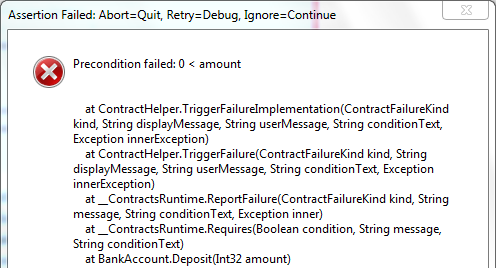
\includegraphics[width=1\columnwidth]{ex2.png}
\end{center}
This failed contract is easily explained if you look at the code in 
\code{Deposit}:
\begin{lstlisting}
    public virtual void Deposit(int amount) {
      Contract.Requires(0 < amount);
      this.balance += amount;
    }
\end{lstlisting}
and then notice that the client was calling it with a negative number.
Fix that in \code{Program.cs} by changing \code{-5} to some positive number.
To see it in action, press \textsf{F10} to start the debugger and have it start at the first line in
the program.
Press \textsf{F10} twice to get to the call to \code{Deposit}.
Now press \textsf{F11} to step into the method call.
Press \textsf{F11} four more times and you'll see that you are now entering the
object invariant:
\begin{center}
  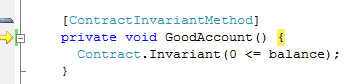
\includegraphics[width=.8\columnwidth]{ex3.png}
\end{center}
Continue execution by pressing \textsf{F5} and the program will run to
completion without an error.

However, if you look at the code in \code{WallStreet.cs}, you'll see that the override
it has for \code{Deposit} does not maintain the invariant of its supertype.
\begin{lstlisting}
    public override void Deposit(int amount) {
      if (100 < amount) {
        this.slushFund += amount;
        this.balance -= amount;
      } else {
        base.Deposit(amount);
      }
    }
\end{lstlisting}
The problem is that runtime checking was enabled for the base class, but not for the subtype.
So now turn on the runtime checking for the project \code{WallStreet} and press \textsf{F5}
to run the program again.
This time you should see another error dialog, this time for the invariant violation:
\begin{center}
  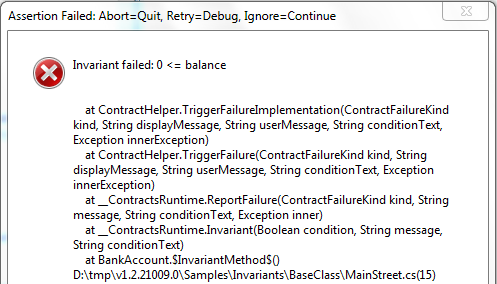
\includegraphics[width=1\columnwidth]{ex4.png}
\end{center}
Note that the invariant check is injected into the subtype even though it has no contracts
at all --- not even a reference to the contract library!

The subtle point that is important to realize is that if you go back to the settings for
the \code{BasicBankAccount} project and now turn {\em off} the runtime checking, then even
though runtime checking is turned on for \code{WallStreet}, the invariant check will not
be injected into the code and no invariant violation will be found.


\end{document}
